% Figure 1, drawn in TikZ. Compiled standalone to figures/idea.pdf (make idea) and included by main.tex.
\documentclass[tikz,border=2pt]{standalone}
% reproducible builds: no dates or random IDs in the PDF
\ifdefined\pdfinfoomitdate \pdfinfoomitdate=1 \fi
\ifdefined\pdftrailerid \pdftrailerid{} \fi
\ifdefined\pdfsuppressptexinfo \pdfsuppressptexinfo=-1 \fi
\usepackage[T1]{fontenc}
\usepackage{mathptmx}
\usepackage[scaled=0.9]{helvet}
\usetikzlibrary{arrows.meta,positioning,calc,shapes.geometric}
\definecolor{goodblue}{HTML}{2A78D6}
\definecolor{badorange}{HTML}{EB6834}
\definecolor{ntpaqua}{HTML}{1BAF7A}
\definecolor{custA}{HTML}{6250D6}
\definecolor{custB}{HTML}{EDA100}
\definecolor{custC}{HTML}{E87BA4}
\definecolor{inktwo}{HTML}{52514E}
\begin{document}
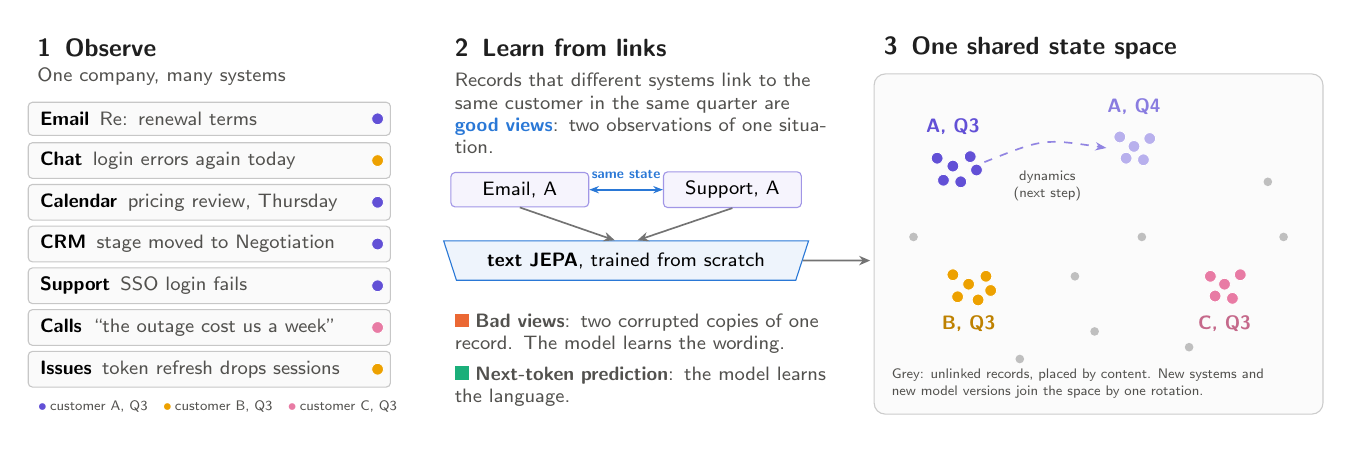
\begin{tikzpicture}[x=1cm,y=1cm,font=\sffamily\scriptsize,
  card/.style={draw=black!22,fill=black!2,rounded corners=1.5pt,minimum width=4.6cm,minimum height=0.42cm,
               inner xsep=3pt,anchor=west,text width=4.3cm,align=left},
  head/.style={font=\sffamily\small\bfseries,anchor=west,text=black!88},
  sub/.style={anchor=west,text=inktwo},
  arr/.style={-{Stealth[length=4pt,width=3.4pt]},line width=0.6pt,draw=black!55},
  dotA/.style={fill=custA,draw=white,line width=0.3pt},
  dotB/.style={fill=custB,draw=white,line width=0.3pt},
  dotC/.style={fill=custC,draw=white,line width=0.3pt}]
% ---------------- panel 1: observe
\node[head] at (0,4.75) {1\enspace Observe};
\node[sub] at (0,4.38) {One company, many systems};
\node[card] (e) at (0,3.85) {\textbf{Email}\enspace\textcolor{inktwo}{Re: renewal terms}};
\node[card] (s) at (0,3.32) {\textbf{Chat}\enspace\textcolor{inktwo}{login errors again today}};
\node[card] (k) at (0,2.79) {\textbf{Calendar}\enspace\textcolor{inktwo}{pricing review, Thursday}};
\node[card] (r) at (0,2.26) {\textbf{CRM}\enspace\textcolor{inktwo}{stage moved to Negotiation}};
\node[card] (t) at (0,1.73) {\textbf{Support}\enspace\textcolor{inktwo}{SSO login fails}};
\node[card] (g) at (0,1.20) {\textbf{Calls}\enspace\textcolor{inktwo}{``the outage cost us a week''}};
\node[card] (j) at (0,0.67) {\textbf{Issues}\enspace\textcolor{inktwo}{token refresh drops sessions}};
\foreach \n in {e,k,r,t} {\fill[dotA] ($(\n.east)+(-0.17,0)$) circle (0.075);}
\foreach \n in {s,j} {\fill[dotB] ($(\n.east)+(-0.17,0)$) circle (0.075);}
\fill[dotC] ($(g.east)+(-0.17,0)$) circle (0.075);
\node[sub,font=\sffamily\tiny] at (0,0.2) {\textcolor{custA}{$\bullet$}\,customer A, Q3\quad \textcolor{custB}{$\bullet$}\,customer B, Q3\quad \textcolor{custC}{$\bullet$}\,customer C, Q3};
% ---------------- panel 2: learn from links
\node[head] at (5.3,4.75) {2\enspace Learn from links};
\node[sub,text width=4.75cm,align=left,anchor=north west] at (5.3,4.55)
  {Records that different systems link to the same customer in the same quarter are \textbf{\textcolor{goodblue}{good views}}: two observations of one situation.};
\node[draw=custA!60,fill=custA!6,rounded corners=1.5pt,minimum width=1.75cm,minimum height=0.42cm] (v1) at (6.25,2.95) {Email, A};
\node[draw=custA!60,fill=custA!6,rounded corners=1.5pt,minimum width=1.75cm,minimum height=0.42cm] (v2) at (8.95,2.95) {Support, A};
\draw[{Stealth[length=3.5pt]}-{Stealth[length=3.5pt]},line width=0.6pt,draw=goodblue] (v1) -- node[above=0.5pt,text=goodblue,font=\sffamily\tiny\bfseries]{same state} (v2);
\node[trapezium,trapezium angle=72,draw=goodblue,fill=goodblue!8,minimum width=3.6cm,minimum height=0.5cm,
      shape border rotate=180] (enc) at (7.6,2.05) {\textbf{text JEPA}, trained from scratch};
\draw[arr] (v1.south) -- ($(enc.north west)!0.22!(enc.north east)$);
\draw[arr] (v2.south) -- ($(enc.north west)!0.78!(enc.north east)$);
\node[sub,text width=4.75cm,align=left,anchor=north west] at (5.3,1.5)
  {\textcolor{badorange}{\rule{5pt}{5pt}}\ \textbf{Bad views}: two corrupted copies of one record. The model learns the wording.\\[3pt]
   \textcolor{ntpaqua}{\rule{5pt}{5pt}}\ \textbf{Next-token prediction}: the model learns the language.};
% ---------------- panel 3: state space
\node[head] at (10.75,4.75) {3\enspace One shared state space};
\draw[rounded corners=4pt,draw=black!20,fill=black!1.5] (10.75,0.1) rectangle (16.45,4.42);
\draw[arr] (enc.east) -- (10.7,2.05);
% unlinked records (grey), drawn first
\foreach \x/\y in {14.15/2.35,13.3/1.85,15.75/3.05,11.25/2.35,14.75/0.95,13.55/1.15,15.95/2.35,12.6/0.8}{\fill[black!25] (\x,\y) circle (0.055);}
% customer A, Q3
\foreach \dx/\dy in {0/0,0.22/0.12,-0.2/0.1,0.1/-0.2,-0.12/-0.18,0.3/-0.05}{
  \pgfmathsetmacro{\x}{11.75+\dx}\pgfmathsetmacro{\y}{3.25+\dy}
  \fill[dotA] (\x,\y) circle (0.075);}
\node[text=custA,font=\sffamily\scriptsize\bfseries] at (11.75,3.75) {A, Q3};
% customer A, Q4
\foreach \dx/\dy in {0/0,0.2/0.1,-0.18/0.12,0.12/-0.17,-0.1/-0.15}{
  \pgfmathsetmacro{\x}{14.05+\dx}\pgfmathsetmacro{\y}{3.5+\dy}
  \fill[fill=custA!45,draw=white,line width=0.3pt] (\x,\y) circle (0.075);}
\node[text=custA!75,font=\sffamily\scriptsize\bfseries] at (14.05,4.0) {A, Q4};
\draw[-{Stealth[length=4pt]},dashed,line width=0.6pt,draw=custA!70] (12.15,3.3) .. controls (12.9,3.6) .. (13.7,3.48);
\node[text=inktwo,font=\sffamily\tiny,align=center] at (12.95,3.0) {dynamics\\(next step)};
% customer B, Q3
\foreach \dx/\dy in {0/0,0.22/0.1,-0.2/0.12,0.12/-0.2,-0.14/-0.16,0.28/-0.08}{
  \pgfmathsetmacro{\x}{11.95+\dx}\pgfmathsetmacro{\y}{1.75+\dy}
  \fill[dotB] (\x,\y) circle (0.075);}
\node[text=custB!80!black,font=\sffamily\scriptsize\bfseries] at (11.95,1.25) {B, Q3};
% customer C, Q3
\foreach \dx/\dy in {0/0,0.2/0.12,-0.18/0.1,0.1/-0.18,-0.12/-0.15}{
  \pgfmathsetmacro{\x}{15.2+\dx}\pgfmathsetmacro{\y}{1.75+\dy}
  \fill[dotC] (\x,\y) circle (0.075);}
\node[text=custC!85!black,font=\sffamily\scriptsize\bfseries] at (15.2,1.25) {C, Q3};
\node[text=inktwo,font=\sffamily\tiny,align=left,anchor=south west] at (10.85,0.18)
  {Grey: unlinked records, placed by content. New systems and\\new model versions join the space by one rotation.};
\end{tikzpicture}
\end{document}
